\chapter{protocol}

	The commitment tree is a tree where each vertex has an associated label representing the data that is passed on to its parent. The messages have the following format: 
	\textit{MESSAGE}
	\newline
	
	\begin{tabular}{ | l | l | l | l |}
		\hline
		ID & COUNT & VALUE & COMMITMENT \\
		\hline
		20 bits & 21 bits & 20 bits & 256 bits\\
		\hline
	\end{tabular}
	\newline
	\newline
	\textit{SIGNATURE (MESSAGE)}
	\newline

	\begin{tabular}{ |l| }
		\hline
		Encryption$_{secret-key_{node}}$( HASH ( MESSAGE ) )\\
		\hline
		500 bits\\
		\hline
	\end{tabular}
	\newline
	\newline
	\textit{CERTIFICATES}
	\newline

	\begin{tabular}{ | l | l | l | }
		\hline
			Public key  & Signature & ID \\
		\hline
			1000 bits & 500 bits & 20 bits \\
		\hline

	\end{tabular}

	\newpage

\section{Aggregation-Commit Phase}
	In this phase, the network constructs a commitment structure. 
	First, the sensor nodes at the highest depth in the aggregation tree (leaf nodes) send their \payloads,defined according to Definition \ref{def:ct}, to their parents in the aggregation tree.
	Each internal sensor node in the aggregation tree performs an aggregation operation whenever it receives \payloads\  from all of its children.
	Whenever a sensor node performs an aggregation operation, it creates a commitment to the set of inputs used to compute the aggregate by computing a hash over all the inputs (including the commitments that were computed by its children). 
	Both the aggregation result and the commitment creates a \payload\ for the aggregator.
	Then the \payload, with the signature of the \payload\ signed by the sensor node are passed on to the parent of the sensor node.
	Once the final \payloads\  and the signatures of those \payloads\  are sent to the \bs, if an adversary tries to claim a different commitment structure it gets caught during the verification phase.
	Our algorithm generates perfectly balanced binary trees to create commitment forests which saves the bandwidth in the verification phase compared to other approaches.

	\begin{definition}\cite{chan2006secure}\label{def:ct}
		A \textbf{\textit{commitment tree}} is a logical tree build on top of an \textbf{\textit{aggregation tree}} where each vertex has an associated \payload\ to it, representing data being passed on to its parent. The \payload\ has the following format:

		$\{\ id,\ count,\ value,\ commitment\ \}$\\
		Where $id$ is the unique identity number of the node; $count$ is the number of leaf vertices in the subtree rooted at this vertex; $value$ is the aggregate computed over all the leaves rooted in the subtree; and commitment is the cryptographic commitment.

	\end{definition}

	Our \payload\ format is different than the label format in \cite{chan2006secure}.
	The \payload\ format adds an ID field and removes the complement field from the label. 
	Our protocol helps detecting an adversary, to achieve this we send the signature of the \payload. 
	And to verify the signature, the verifier needs the ID of that node.
	The complement field was used to verify the upper bound on the aggregation result by the \bs.
	We claim that the result can be achieved by sending count only, sending complement was redundant and no longer required.     

	There is one leaf vertex $s.v$ for each sensor node $s$ with the \payload,
	\begin{equation}\label{eq:vertex}
		s.p = \{\ s.id,\ 1,\ s.value,\ Hash( N\ ||\  s.id\ ||\  1\  ||\  s.value\ ) \} 
	\end{equation}
	where $N$ is the query nonce which is disseminated with each query.

	Internal vertices represent aggregation operations, and have \payloads\  that are defined based on their children. Suppose an internal vertex has child vertices $s_{1}.v, s_{2}.v,\dotsc, s_{q}.v$ with the following \payloads: $s_{1}.p, s_{2}.p,\dotsc, s_{q}.p$, where
	\begin{equation}\label{def:internal-vertice}
		s_{i}.p = \{\ s_{i}.id,\ s_{i}.count,\ s_{i}.value,\ s_{i}.commitment\ \}
	\end{equation}
	Then the internal vertex has \payload, 
	\begin{equation}
		s.p = \{\ id,\ count,\ value,\ commitment\ \} 
	\end{equation}
	\begin{equation}
		id = s.id 
	\end{equation}	
	\begin{equation}
		count = \sum\limits_{i=1}^q {s_{i}.count}		
	\end{equation}
	\begin{equation}
		value = \sum\limits_{i=1}^q {s_{i}.value}		
	\end{equation}
	\begin{equation}
		commitment = H (N\ ||\ id\ ||\ count\ ||\ value\ ||\textcolor{red}{\ s_{1}.p\ ||\ s_{2}.p\ || \dotsb ||\ s_{q}.p})		
	\end{equation}

	Every \payload\ has an associated signature to it, which is the encryption of the hash of the \payload\ using node's private key. For example, signature associated with equation \ref{eq:vertex} is the following:  
	\begin{equation}
		s.sign(p) = E_{s.{private-key}}(H (s.p))
	\end{equation}
	We use elliptic curve cryptography to minimize keys and signatures bit size. 
	Also, we use the collision resistant hash function so it's impossible for an adversary to tamper with any of the commitments once they are created.	

	There is a mapping between the vertices in the commitment tree and the sensor nodes in the aggregation tree, a vertex is a logical element while a node is a physical device.
	To avoid confusion, we use the term vertex for the members in the commitment tree and node for the members of the aggregation tree.
	
	The \at\ is a rooted tree created from the network graph. 
	To create an optimal \at\ from the given network graph is outside the scope of this thesis.
	Our algorithm takes any arbitrary \at\ as an input. 
	One possible \at\ for given network graph in Figure \ref{fig:ng} is shown in the Figure \ref{fig:at}.
	We use the term \bs\  for the trusted third party. In Figure \ref{fig:at} $BS$ is the \bs.
		
	\begin{figure}[hp]
		\centering
		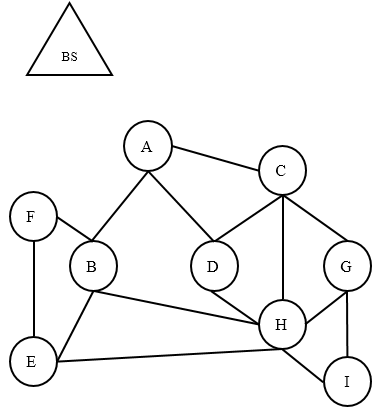
\includegraphics[scale = 0.5]{images/network-graph.png}\\
		\caption{Network graph}
		\label{fig:ng}
	\end{figure}

	\begin{figure}[hp]
		\centering
		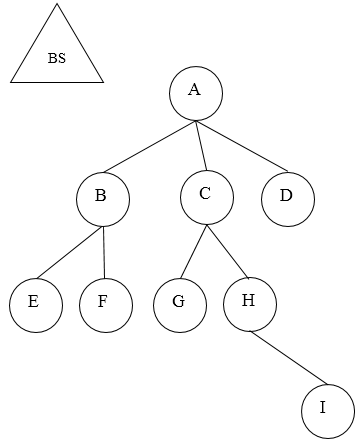
\includegraphics[scale = 0.5]{images/aggregation-tree.png}\\
		\caption{Aggregation tree for network graph in figure \ref{fig:ng}}
		\label{fig:at}
	\end{figure}

	Each sensor node $s$ has it's own sensor reading $s.value$. The \bs\ is interested in overall behavior of the network, which is some function $f$ of all $n$ sensor readings.
	\begin{equation}
		f(s_{1}.value, s_{2}.value, s_{3}.value, \dotsc, s_{n}.value)
	\end{equation}
	We discuss the case for the \textit{SUM} function, but the protocols discussed here can be applied to many other functions with little or no modification. 
	\begin{equation}
		\textit{SUM} = \sum\limits_{i=1}^n s_{i}.value
	\end{equation}

	\subsection{No aggregation approach}
		One way to calculate the \textit{SUM} is to send all the $n$ \payloads\ to the \bs.
		It means all the internal nodes in the network send all the \payloads\ received from their descendants to their parent.
		Once the \bs\ has all $n$ \payloads, it computes the summation.
		For any given node, the \inforate\ is 1. \inforate\ is defined in Definition \ref{def:ir}.\\
		Advantages:
		\begin{itemize}
			\item Perfectly secure.
		\end{itemize}
		Disadvantages:
		\begin{itemize}
			\item Requires $O(n)$ bandwidth between the \bs and the \bs.
			\item Requires $O(d)$ bandwidth between the internal node and its parent, where $d$ is the number of descendants for a given node.
			\item Very high \inforate.
		\end{itemize}
			
	\begin{definition}\label{def:ir}
		The \inforate\ for a particular node is the \payloads\ ratio, number of \payloads\ sent / number of \payloads\ received.
	\end{definition}

	\subsection{Naive approach}
		Another way to calculate the \textit{SUM} is to send only one \payload\ to the \bs.
		It means all the internal nodes in the network, after receiving readings from all of their children, does the summation including their own reading and then pass the resulted \payload\ to their parents' as shown in Figure \ref{fig:naive-commitment-tree}.
		For any given node, the \inforate\ is $1 / (c + 1)$, where $c$ is the number of children for the give node.\\
		Advantages:
			\begin{itemize}
				\item Optimal \inforate.
			\end{itemize}
		Disadvantages:
			\begin{itemize}
				\item Makes aggregated value more vulnerable to various security attacks.
				\item Requires more bandwidth in the verification phase.
			\end{itemize}
		\begin{figure}[hp]
			\centering
			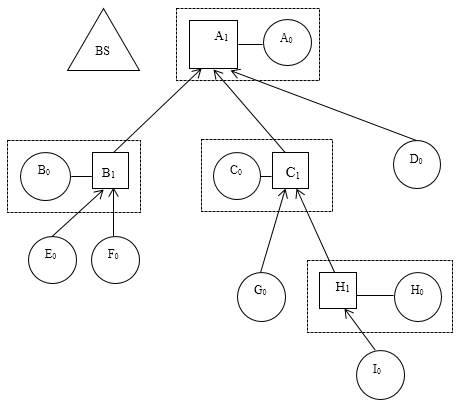
\includegraphics[scale = 0.6]{images/naive-commitment-tree.png}\\
			\caption{Naive commitment tree}
			\label{fig:naive-commitment-tree}
		\end{figure}

	\subsection{Aggregate-commit approach}
		The no aggregation and naive approaches are two extreme approaches.
		The aggregate-commit approach of \cite{chan2006secure} is between these two extreme cases. It combines the advantages of both the approaches.

		In the naive approach, each sensor node $s$ sends to its parent a single message containing the \payload\ of the root vertex of its commitment subtree $T_{s}$.
		In the aggregate-commit approach, each sensor node $s$ sends the \payloads\ of the root vertices of a set of commitment subtrees $F = \{ T_{1},T_{2},\dotsc,T_{q} \} $, called commitment forest. 

		\begin{definition}\cite{chan2006secure}
			A commitment forest is a set of complete binary commitment trees such that there is	at most one commitment tree of any given height.
		\end{definition}
		The commitment forest with $n$ leaf vertices has the following properties:
		\begin{itemize}
			\item The tallest tree in the forest has height at most $\log(n)$.
			\item There are at most $\log(n)$ trees in the forest.
			\item The \inforate\ is $\log(n+1) / n$.
		\end{itemize}
		We claim that the binary representation of a number $x$ illustrates the forest decomposition of the sensor node $s$, where $x$ = $1\ +$ number of descendants of $s$.
		For example, if sensor node $s$ has $22$ descendants then $x =23$, $(x)_{10}$ = $(10111)_{2}$. 
		It means $s$ has four complete binary trees in its outgoing forest, with the height of four, two, one and zero.
		Note that all the trees in the commitment forest are complete binary trees and no two trees have the same height.
		In the following section we describe how to build commitment forest with an example and also how to reason about commitment forest using binary addition. 

	\subsection{Commitment forest generation}
		The sensor nodes at the highest depth in the aggregation tree (leaf nodes) initiate a single-vertex commitment forest, which they transmit to their parent sensor node.
		Each internal sensor node $s$ initiates a similar single-vertex commitment forest.
		In addition, $s$ also receives commitment 	forests from each of its children.
		Sensor node $s$ keeps track of which root vertices are received from which of its children.
		It then aggregates all the forests to form a new forest as follows.
		
		Suppose $s$ wishes to combine $q$ commitment forests $F_{1}$, $\dotsc$, $F_{q}$ and create an aggregated forest $F$.
		To do so, the sensor node $s$ merges trees with the same height in its forests by creating a new tree with the height incremented by $1$. 
		It repeats this process until no two trees in its forest have the same height. 
		Let $T_{1}, T_{2}$ have the height $h$, where $h$ is the smallest height in $F$.
		The sensor node $s$ merges $T_{1}, T_{2}$ into a tree of height $h + 1$ by creating a new vertex according to equation \ref{def:internal-vertice}.
		It repeats this process until all the trees have unique height in the forest.
		An example of the commitment forest generation process for the sensor node $A$ in Figure \ref{fig:at} is illustrated in the Figures \ref{fig:commitment-tree-example-1}, \ref{fig:commitment-tree-example-2}, \ref{fig:commitment-tree-example-3}, \ref{fig:commitment-tree-example-4}.

		In aggregation-commit approach there are at most $\log(n+1)$ commitment trees in each forest transmitted by any sensor node to its parent, which is greater than $1$.
		But all the trees have height less than or equal to $\log(n)$, which makes transmission of off-path values communication efficient which will be discussed in the verification phase.

	\begin{figure}[hp]
		\centering
		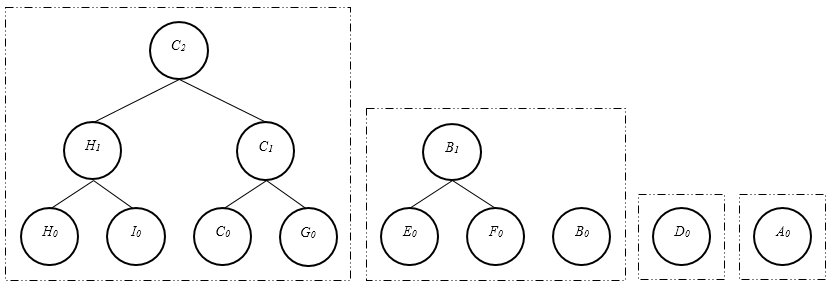
\includegraphics[scale = 0.7]{images/commitment-tree-example-1.png}\\
		\caption{$A$ receives $C_{2}$ from $C$, $(B_{1},B_{0})$ from $B$, $D_{0}$ from $D$ and generates $A_{0}$. The commitment forest received from a given sensor node is indicated by dashed-line box.}
		\label{fig:commitment-tree-example-1}
	\end{figure}
	The sensor node $A$ receives the following \payloads:
		\begin{equation}
			A_{0} = \{\ A.id,\ 1,\ A.value,\ H  (\ N\ ||\ A.id\ ||\ 1\ ||\ A.value)\ \}\ (internal)
		\end{equation}
		\begin{equation}
			D_{0} = \{\ D.id,\ 1,\ D.value,\ H(\ N\ ||\ D.id\ ||\ 1\ ||\ D.value)\ \}\ (from\ D)
		\end{equation}
		\begin{equation}
			B_{0} = \{\ B.id,\ 1,\ B.value,\ H(\ N\ ||\ B.id\ ||\ 1\ ||\ B.value)\ \}\ (from\ B)
		\end{equation}
		\begin{equation}
			B_{1} = \{\ B.id,\ 2,\ B_{1}.value,\ H(\ N\ ||\ B.id\ ||\ 2\ ||\ B_{1}.value)\ \}\ (from\ B)
		\end{equation}
		\begin{equation}
			C_{2} = \{\ C.id,\ 4,\ C_{2}.value,\ H(\ N\ ||\ C.id\ ||\ 4\ ||\ C_{2}.value)\ \}\ (from\ C)
		\end{equation}

	\begin{figure}[hp]
		\centering
		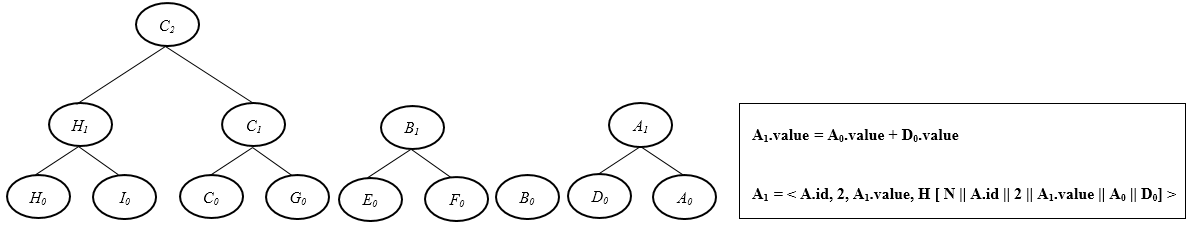
\includegraphics[scale = 0.7]{images/commitment-tree-example-2.png}\\
		\caption{First Merge: $A_{1}$ vertex created by A}
		\label{fig:commitment-tree-example-2}
		\begin{equation}
			A_{1} = \{\ A.id,\ 2,\ A_{1}.value,\ H(\ N\ ||\ A.id\ ||\ 2\ ||\ A{1}.value\ )\ \}
		\end{equation}
		\begin{equation}
			A_{1}.value = A.value + D.value
		\end{equation}
	\end{figure}

	\begin{figure}[hp]
		\centering
		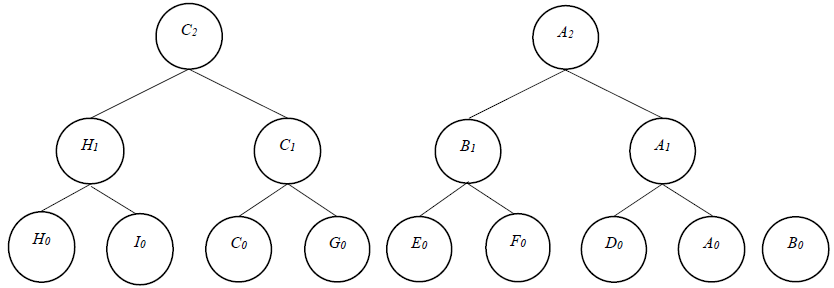
\includegraphics[scale = 0.7]{images/commitment-tree-example-3.png}\\
		\caption{Second Merge: $A_{2}$ vertex created by A}
		\label{fig:commitment-tree-example-3}
		\begin{equation}
			A_{2} = \{\ A.id,\ 4,\ A_{2}.value,\ H(\ N\ ||\ A.id\ ||\ 4\ ||\ A_{2}.value\ )\ \} 
		\end{equation}
		\begin{equation}
			A_{2}.value = A_{1}.value + B_{1}.value
		\end{equation}
	\end{figure}

	\begin{figure}[hp]
		\centering
		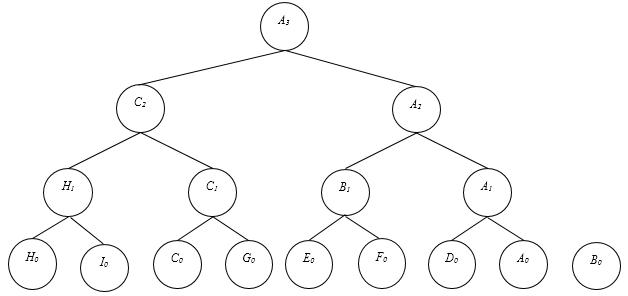
\includegraphics[scale = 0.7]{images/commitment-tree-example-4.png}\\
		\caption{Third Merge: $A_{3}$ vertex created by A}
		\label{fig:commitment-tree-example-4}
		\begin{equation}
			A_{3} = \{\ A.id,\ 8,\ A_{3}.value,\ H(\ N\ ||\ A.id\ ||\ 8\ ||\ A_{3}.value\ )\ \} 
		\end{equation}
		\begin{equation}
			A_{3}.value = A_{2}.value + C_{2}.value
		\end{equation}
	\end{figure}

	% \subsection{Binary representation of Aggregation-Commit approach}
	The commitment forest generation process for the sensor node $A$ in Figure \ref{fig:at}, can be illustrated in the binary format as follows: 
	\[ 
		\begin{array}{lcccc}
			\mbox{Carry} & 0 & 1 & 1 & 0\\
			\hline
			\mbox{B's forest} & 0 & 0 & 0 & 1 \\
			\mbox{ } & 0 & 0 & 1 & 0 \\
			\hline
			\mbox{C's forest} & 0 & 1 & 0 & 0 \\
			\hline
			\mbox{D's forest} & 0 & 0 & 0 & 1 \\
			\hline
			\mbox{A's payload} & 0 & 0 & 0 & 1 \\
			\hline
			\mbox{Aggregation} & 1 & 0 & 0 & 1 
		\end{array}
	\]
	The sensor node $A$ receives $B, C, D's $ forests and creates its own single vertex forest. Creating a commitment forest is similar to doing summation on the received forests' binary format.
	Also, generating a carry in the summation is equivalent to creating a new vertex in the commitment forest by merging two trees. 
	Also, the carry is always generated of the aggregation node.
	In the analysis chapter, we show that for the aggregation node being root in as many as possible trees is communication efficient.

	Observe that $A$ has several ways of doing the summation.
	For example, while adding lowest significant bits it has $1's$ at three places. The aggregation node $A$ can use any two $1's$ to generate a carry. If $A$ uses $1's$ from $B, D's$ forest than in the final aggregation lowest significant bit represents $A's$ vertex. 
	If vertex related to node is represented by its letter than above summation process can be represented in the following ways.
	\[ 
		\begin{array}{lcccclcccclcccc}
			\mbox{Carry} & 0 & A & A & 0\  \vline & 0 & A & A & 0\ \vline & 0 & A & A & 0\ \\
			\hline
			\mbox{B's forest} & 0 & 0 & 0 & 1\ \vline & 0 & 0 & 0 & 1\ \vline & 0 & 0 & 0 & 1\ \\
			\mbox{ } & 0 & 0 & 1 & 0\ \vline & 0 & 0 & 1 & 0\ \vline & 0 & 0 & 1 & 0\ \\
			\hline
			\mbox{C's forest} & 0 & 1 & 0 & 0\ \vline & 0 & 1 & 0 & 0\ \vline & 0 & 1 & 0 & 0\ \\
			\hline
			\mbox{D's forest} & 0 & 0 & 0 & 1\ \vline & 0 & 0 & 0 & 1\ \vline & 0 & 0 & 0 & 1\ \\
			\hline
			\mbox{A's payload} & 0 & 0 & 0 & 1\ \vline & 0 & 0 & 0 & 1\ \vline & 0 & 0 & 0 & 1\ \\
			\hline
			\mbox{Aggregation} & A & 0 & 0 & A\ \vline & A & 0 & 0 & B\ \vline & A & 0 & 0 & D\ \\  
		\end{array}
	\]	

\newpage
\begin{algorithm}[H]\label{number3} \caption{CommitmentTreeGeneration}
	\begin {algorithmic}[1]

		\STATE d = \at.MaxDepth
		\WHILE {d $\geq$ 0}

			\FORALL {\node \   $\in$ \at.depth }

			\STATE \node.\forest = NULL
					\STATE Create (\node.\msg, \sign $_{\cal{N}}$(\node.\msg))
					\STATE Attach (\node.\msg, \sign $_{\cal{N}}$(\node.\msg)) to \node.\forest
					
					\IF {\node.\children \ $\neq$ \ 0}

						\FORALL {\child \ $\in$ \node.\children }

							\FORALL {tree root \treeRoot \ $\in$ \child.\forest}

								\IF {\node \ has \treeRoot.\cert\  (else get \treeRoot.\cert )} 

									\IF {\node verifies \treeRoot.\msg\ (else raise an alarm)}

										\STATE Add \treeRoot \ into \node.\forest
										
									\ENDIF
								
								\ENDIF

							\ENDFOR

							\STATE \node.\forest \ =	CommitmentTreeCoding ( \node.\forest \ ) 
						
						\ENDFOR
		
					\ENDIF


			\ENDFOR

			\STATE {d = d - 1 }

		\ENDWHILE
	\end{algorithmic}
\end{algorithm}

\begin{algorithm}[H]\caption{CommitmentTreeCoding}
	\begin{algorithmic}[1]

		\STATE \temp \ = SortLinkedList( \node, \node.\forest \ ) /*returns head of the linked list*/

		\WHILE {\temp.\nextTree \ $\neq$ \ 0}

			\IF {\temp.\height \ $\neq$ \ \temp.\nextTree.\height } 
				\STATE \temp \ = \temp.\nextTree
			\ELSE

				\STATE Create an aggregation node \aggregator 
				\STATE \aggregator.\height \ = \temp.\height \ + 1
				\STATE \aggregator.\lc \ = \temp
				\STATE \aggregator.\rc \ = \temp.\nextTree
				\STATE Insert \aggregator \ into \node.\forest
				\STATE Remove \temp
				\STATE Remove \temp.\nextTree
				\STATE \temp \ = SortLinkedList( \node, \node.\forest \ )

			\ENDIF

		\ENDWHILE		

		\STATE return \temp

	\end{algorithmic}

\end{algorithm}


\textit{Properties of commitment tree and aggregation tree}

	If you have $O(n)$ children then you need at least $\Omega(n)$ \& at max $O(n\log(n))$ certificates.

	If you have $O(n)$ descendants then you need $\Omega(\log(n))$  \& at max $O(n\log(n))$ certificates.


\section{Advantages of this protocol}
\section{Disadvantages of this protocol}